\chapter{Compact Muon Solenoid}

\section{Introduction}
About 100 meters below the town of Cessy, France at Point 5 is the Compact Muon Solenoid (CMS).  The CMS is a general purpose detector weighing 14,000 tonnes with a length of 28.7 meters and a 15.0-meter diameter that was designed to accurately measure the energy and momentum of particles produced in the proton-proton or heavy-ion collisions at the LHC \cite{Collaboration_2008}.  A perspective view of of the detector is shown in Figure \ref{fig:cmsschematic}.  In order to get a full picture of what is being produced by the collisions the CMS detector must be able identify the resulting particles as well as accurately measure their energy and momentum.  For this reason the detector was designed to be a collection of specialized sub-detectors, each of which contributes data used in the reconstruction of a collision.  
\begin{figure}[h]
	\centering
	\includegraphics[width=0.7\linewidth]{Figures/cms_schematic}
	\caption{Schematic of CMS detector \cite{Sakuma_2014}}
	\label{fig:cmsschematic}
\end{figure}

At the heart of the CMS detector is a 3.8-Tesla magnetic field produced by a superconducting solenoid.  Inside the 6-meter diameter solenoid are three layers of sub-detectors.  These make up the inner detector and are, in order from innermost to outermost, the silicon tracker, the electromagnetic calorimeter (ECAL), and the hadronic calorimeter (HCAL).  Outside the solenoid is the muon system.  A transverse slice of the detector (Figure \ref{fig:cmsslicewhitecolourfrench291016}) shows the sub-detectors and how different types of particles interact with with them.  Table \ref{table:subdetsignals} shows a summary of which sub-detectors are expected to produce signals for different types of particles.

\begin{figure}[h]
	\centering
	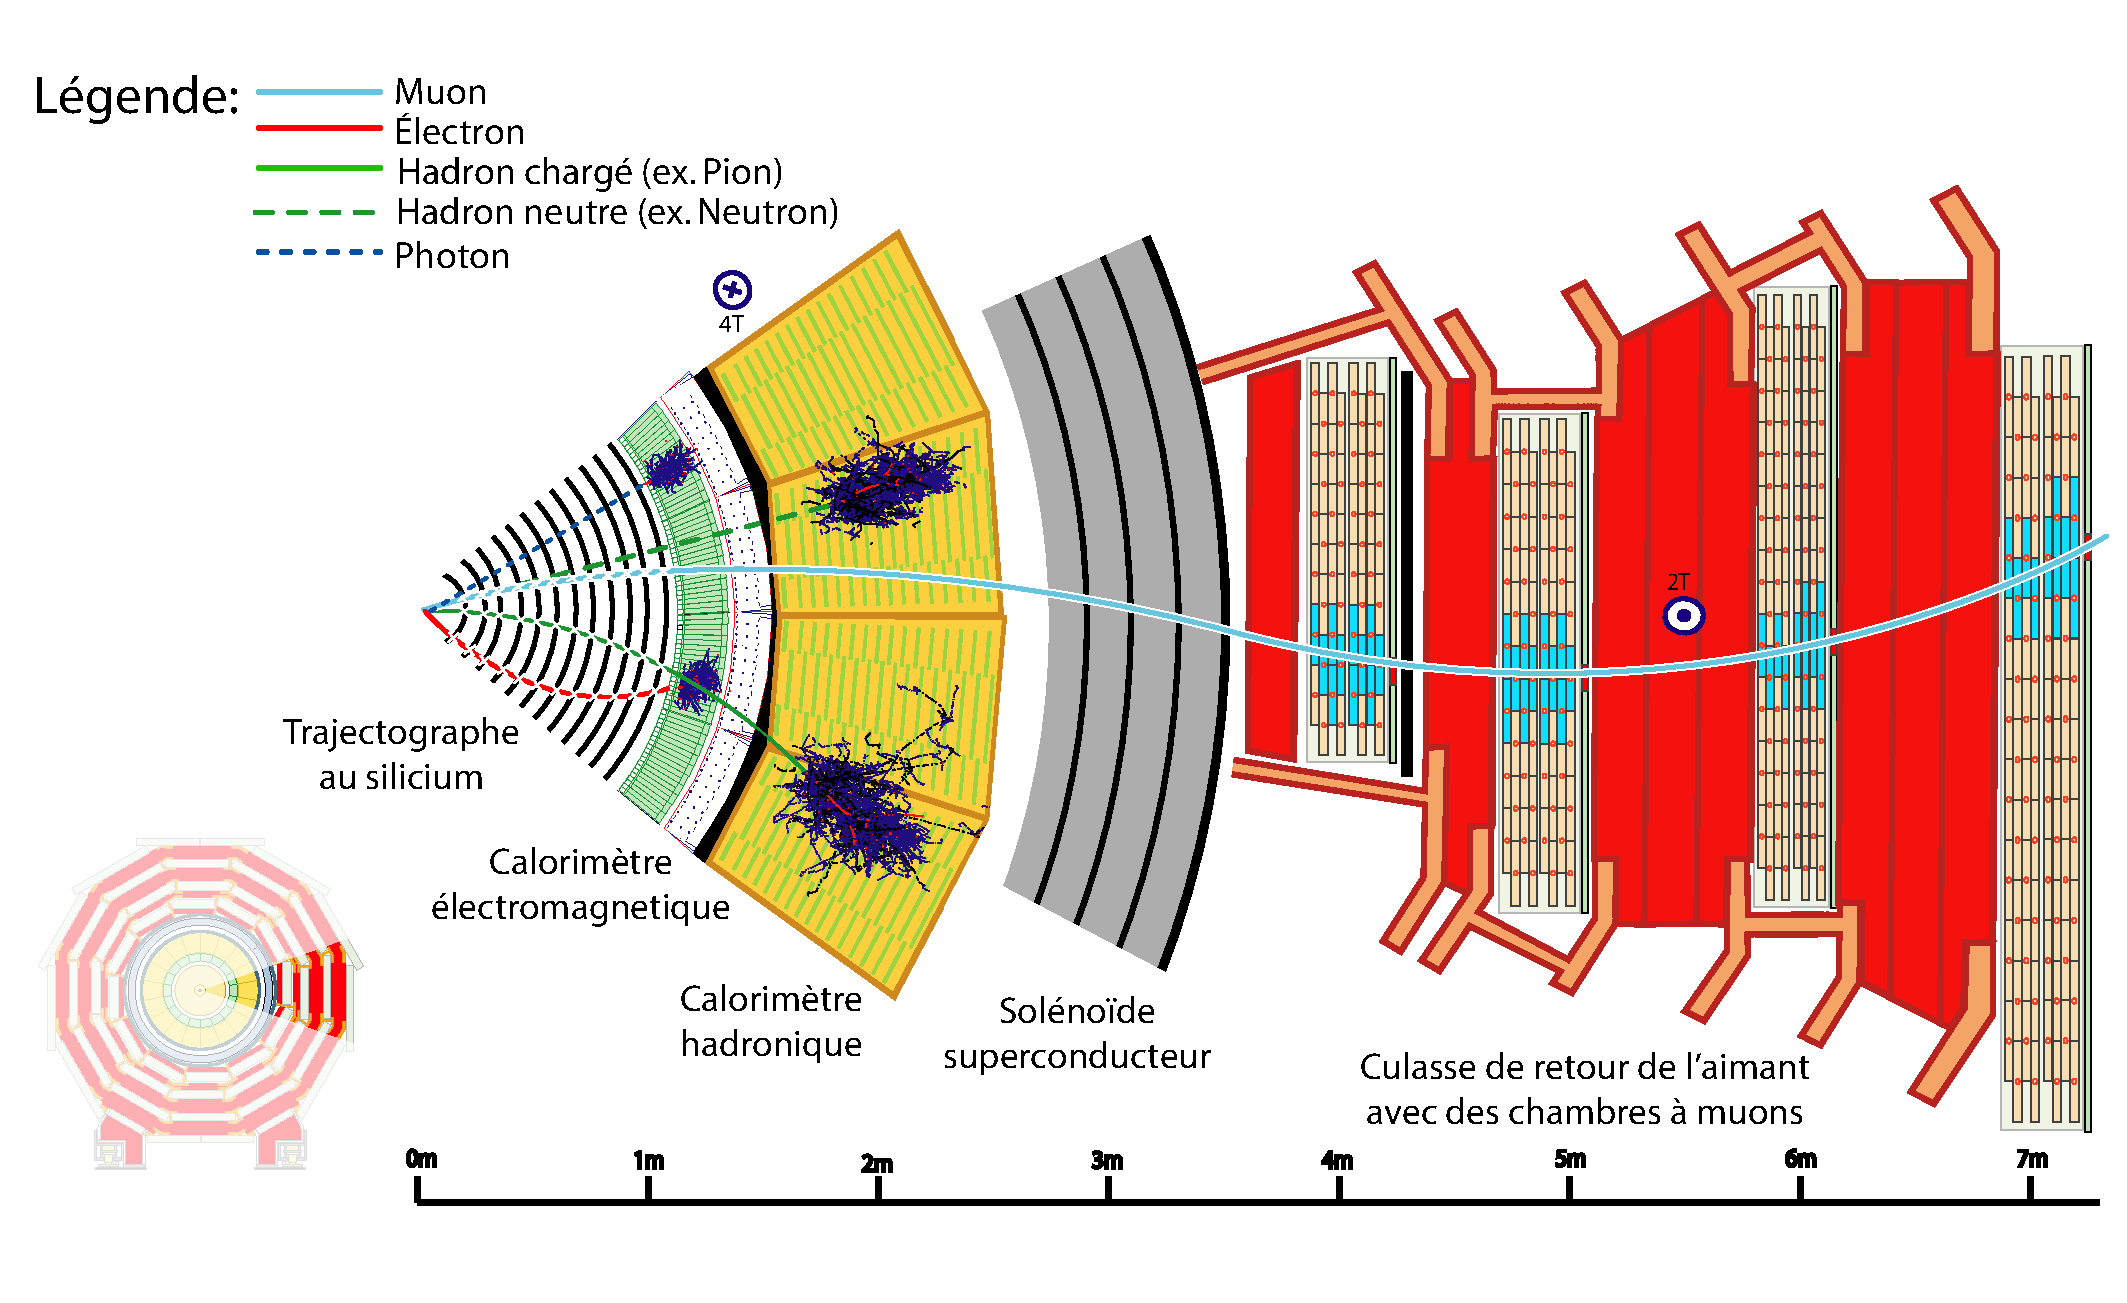
\includegraphics[width=0.7\linewidth]{Figures/CMS_slice_white_colour_french_291016}
	\caption{Transverse slice of the CMS detector\cite{Barney:2628641}.}
	\label{fig:cmsslicewhitecolourfrench291016}
\end{figure}



\begin{table}[h]
	\centering
\begin{tabular}{|c|c|c|c|c|}
	\hline 
	Particle & Tracker & ECAL & HCAL & Muon \\ 
	\hline 
	Photons & No & Yes & No & No \\ 
	\hline 
	Electrons & Yes & Yes & No & No \\ 
	\hline 
	Hadrons (charged) & Yes & No & Yes & No \\ 
	\hline 
	Hadrons (neutral) & No & No & Yes & No \\ 
	\hline 
	Muons & Yes & No & No & Yes \\ 
	\hline 
	Invisible ($\nu$, SUSY, etc) & No & No & No & No \\ 
	\hline 
\end{tabular} 
\caption{Summary of signals expected for each particle type in each sub-detector}
\label{table:subdetsignals}
\end{table}


\section{Coordinate System}
The origin of the coordinate system used by CMS is centered at the nominal collision point in the center of the detector.  A right-handed Cartesian system is used with the x-axis pointing radially inward toward the center of the LHC ring, y-axis pointing vertically upward, and the z-axis pointing tangent to the LHC ring in the counterclockwise direction as viewed from above.  CMS also uses an approximately Lorentz invariant spherical coordinate system spanned by three basis vectors.  They are the transverse momentum $p_{T}$, pseudorapidity $\eta$, and azimuthal angle $\phi$.  The transverse momentum and azimuthal angle translate to the Cartesian system in the following ways using the x and y-components of the linear momentum:
\begin{equation}
p_{T} = \sqrt{(p_{x})^{2} + (p_{y})^{2}}
\end{equation}
\begin{equation}
\phi = tan^{-1}\frac{p_{y}}{p_{x}}
\end{equation}
while the pseudorapidity can be translated using the polar angle $\theta$ relative the positive z-axis as
\begin{equation}
\eta = -ln[tan\frac{\theta}{2}].
\end{equation}


\section{Tracker}
The innermost sub-detector in CMS is the silicon tracker.  The tracker is used to reconstruct tracks and vertices of charged particles.  In order to give precise reconstruction of charged particle trajectories it needs to be position as close as possible to the IP and have high granularity.  The close proximity to the IP requires the materials to be tolerant to the high levels of radiation in that region.  Being the innermost sub-detector it must also minimally disturb particles as they pass through it into the other sub-detectors.  These criteria led to the design of the tracker using silicon semiconductors.

The silicon tracker is made up of two subsystems, an inner pixel detector and an outer strip tracker which are oriented in a cylindrical shape with an overall diameter of 2.4 m and length of 5.6 m centered on the interaction point.  Both subsystems consist of barrel and endcap regions which can be seen in Figure \ref{fig:trackerlayoutv2}.  

\begin{figure}[h]
	\centering
	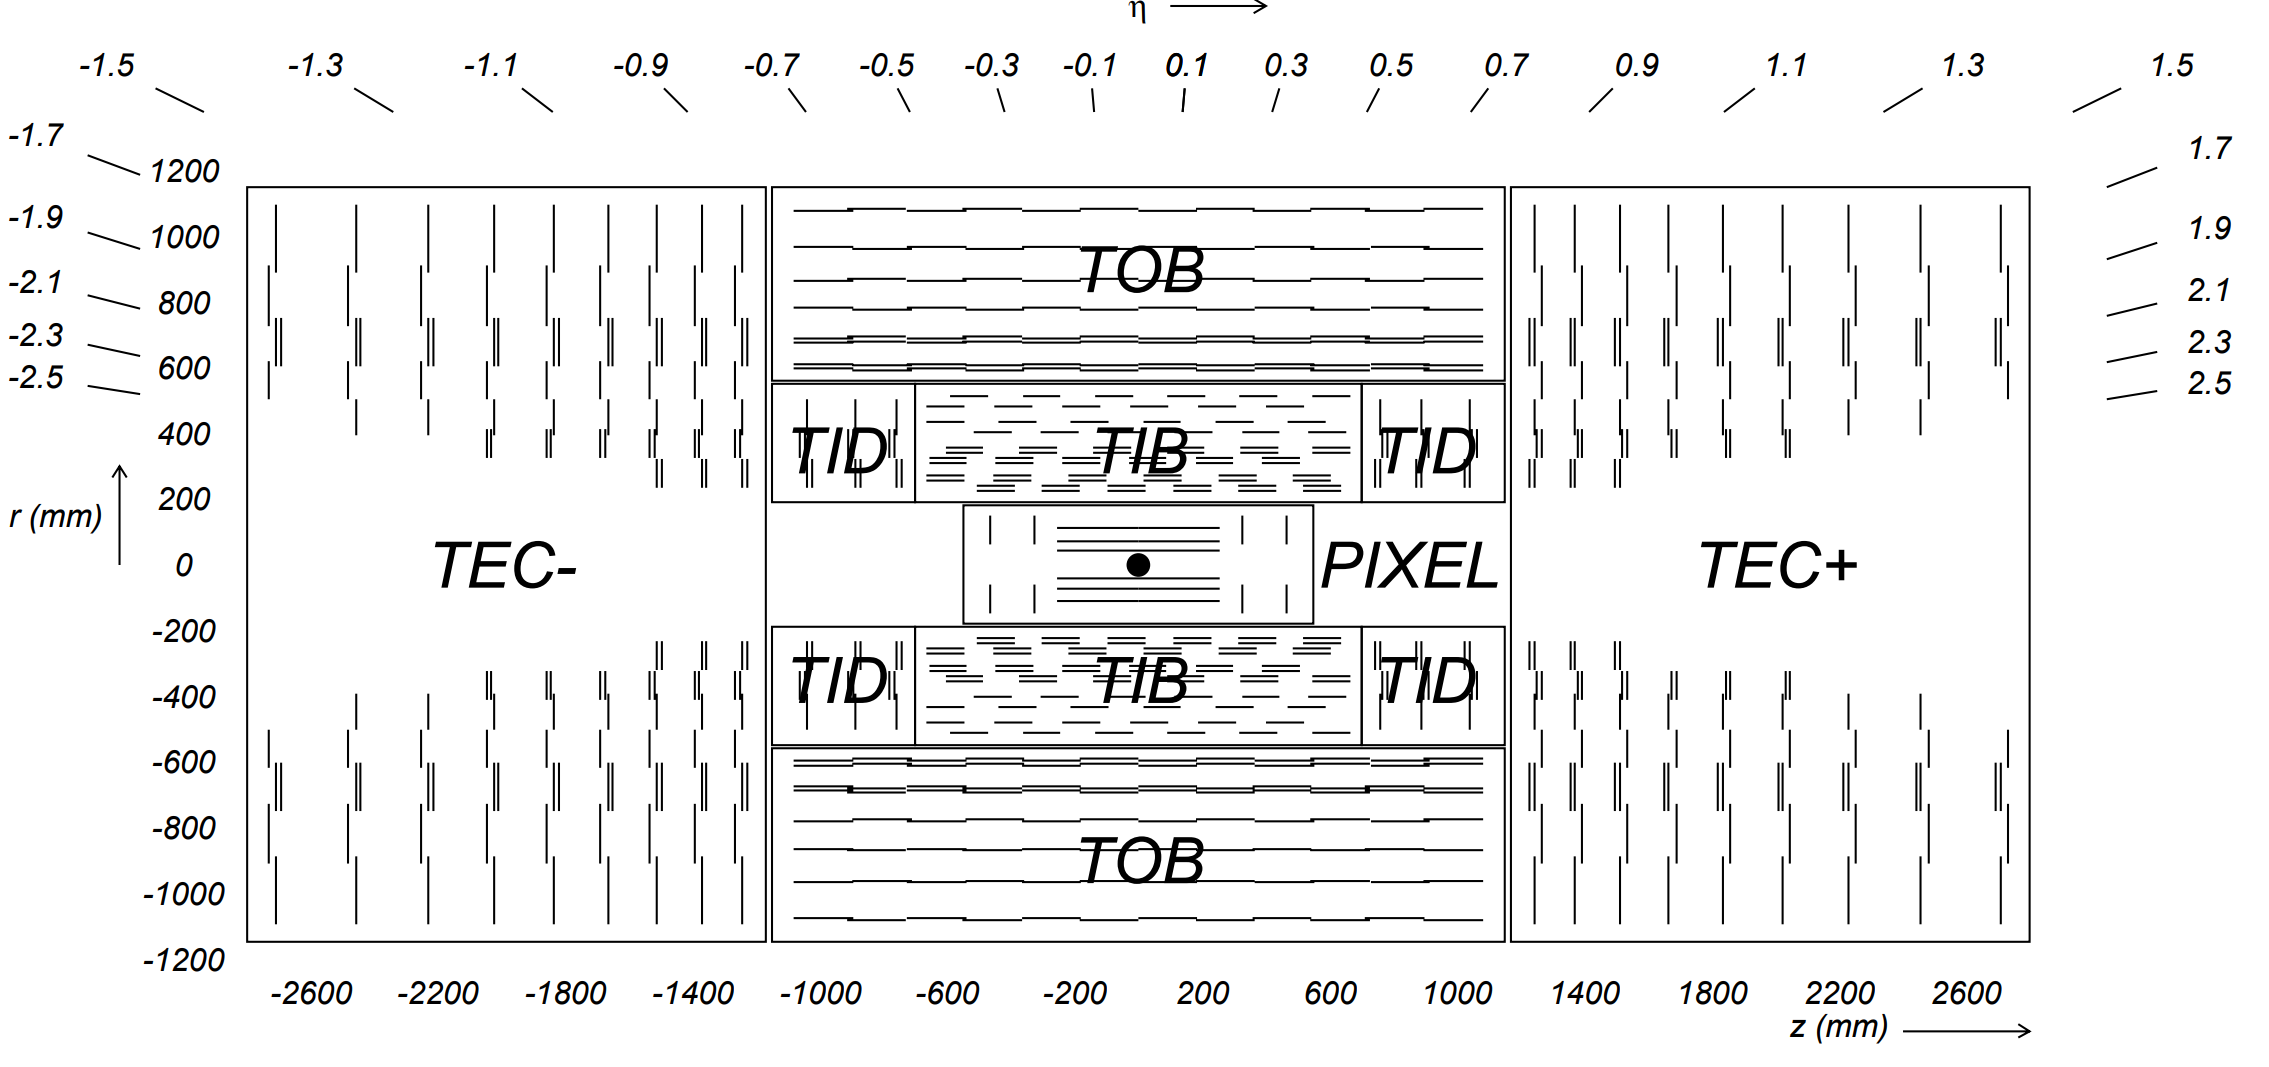
\includegraphics[width=0.7\linewidth]{Figures/TrackerLayout_v2}
	\caption{Cross section (side) of CMS tracker prior to the Phase 1 upgrade during the year-end technical stop of 2016/2017. Each line represents a detector module while double lines indicate back-to-back strip modules. Surrounding the pixel tracker (PIXEL) is the strip detector, which is divided into the Tracker Inner Barrel (TIB), Tracker Outer Barrel (TOB), Tracker Inner Disks (TID), and Tracker Endcaps (TEC). Reprinted from Reference \cite{Chatrchyan:1704291}.}
	\label{fig:trackerlayoutv2}
\end{figure}

\subsection{Pixel Detector}
The pixel detector is the innermost subsystem in the silicon tracker and spans the pseudorapidity range $|\eta|< 2.5$ and is responsible for small impact parameter resolution which is important for accurate reconstruction of secondary vertices \cite{Collaboration_2008}.  In order to produce these precise measurements a very high granularity is required.  In addition to this the proximity to the IP means that one expects there to be high occupancy of the tracker.  These constraints are met by using pixels with a cell size of 100 x 150 $\mu$m$^{2}$.  

The original pixel detector was designed for operation at the nominal instantaneous luminosity of 10$^{34}$ cm$^{-2}$s$^{-1}$ with 25 ns between proton bunch crossings, resulting in on average about 25 proton-proton interactions occurring per bunch crossing or pileup \cite{Chatrchyan:1704291}.  During the LHC technical shutdown of 2016/17, the pixel detector underwent the scheduled Phase 1 upgrade which would allow operation at higher levels of instantaneous luminosity and pileup.  Figure \ref{fig:trackersideview} shows a cross sectional view in the \textit{r-z} plane.  Prior to 2017 there were three barrel layers and two endcap layers on each side which provide three very precise space points for each charged particle.  The upgrade decreased the radius of the innermost barrel layer from 4.4 cm to 3.0 cm and added a fourth barrel layer as well as adding third endcap layer to each side.  Each of the endcap layers consisted of two half-disks populated with pixel modules whereas the upgraded endcap layers were split into inner and outer rings. \cite{Dominguez:1481838}

\begin{figure}[h]
	\centering
	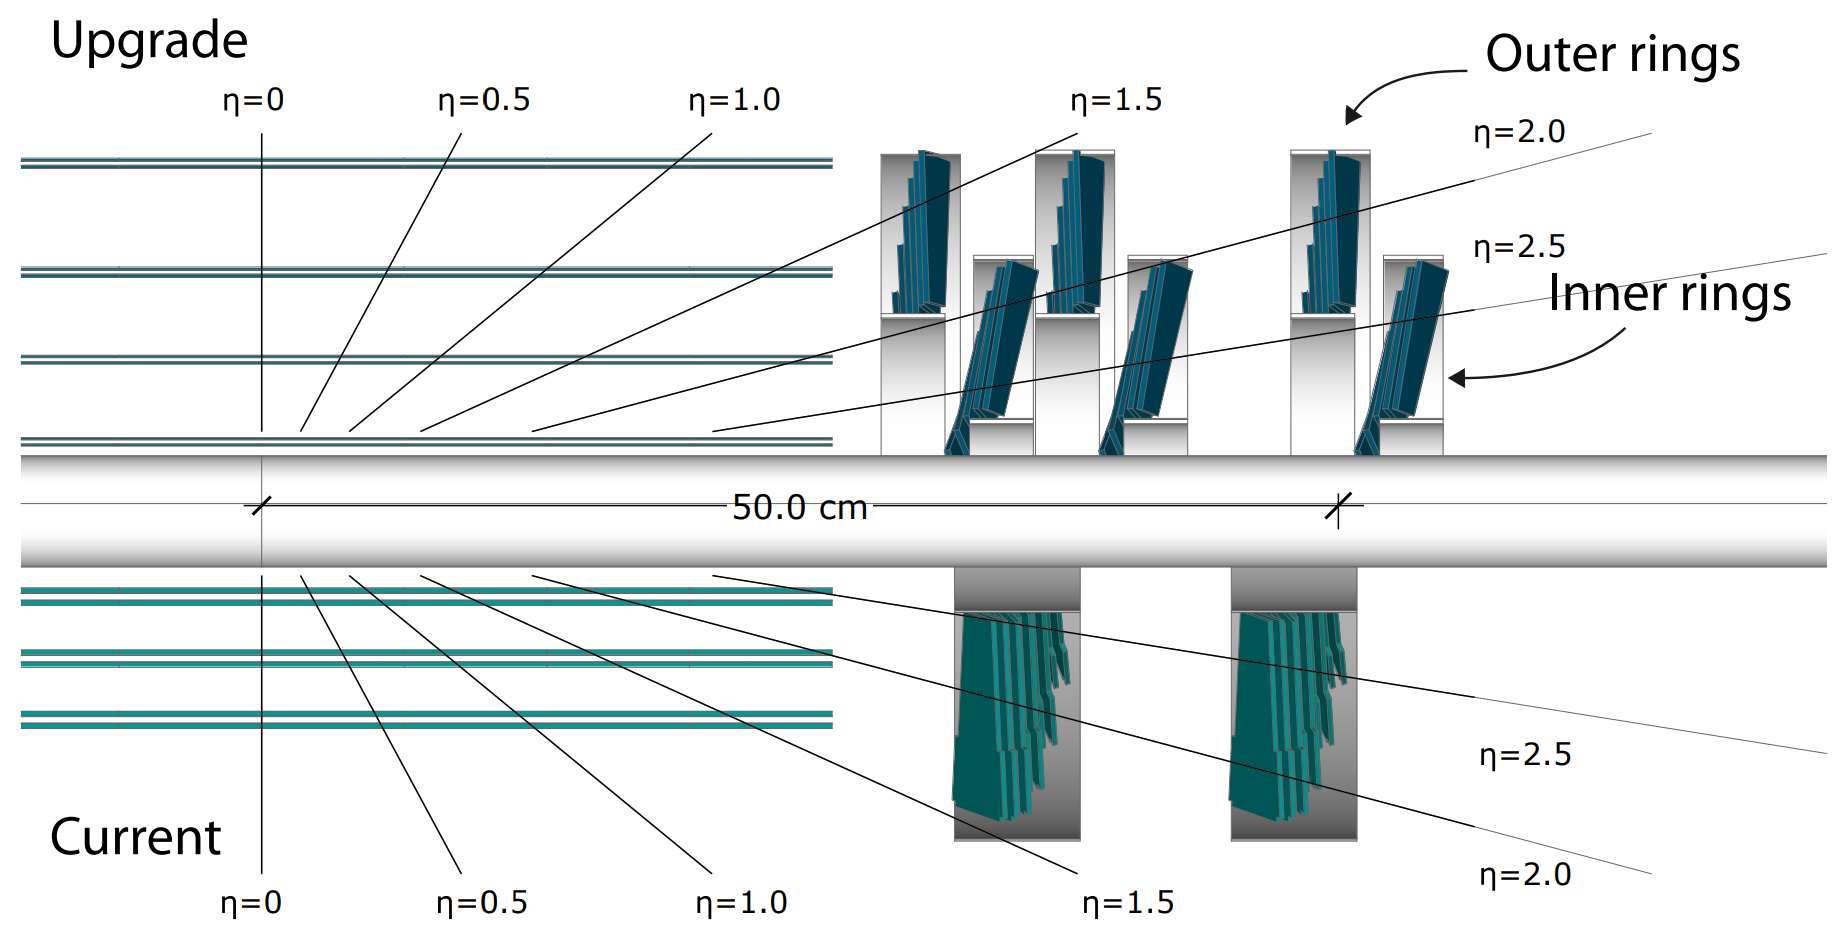
\includegraphics[width=0.7\linewidth]{Figures/Tracker_sideview}
	\caption{Cross section (side) of pixel detector. The lower half , labeled "Current", shows the design prior to 2017 while the upper half, labeled "Upgrade", shows the design after the upgrade. Reprinted from Resource \cite{Dominguez:1481838}}
	\label{fig:trackersideview}
\end{figure}

\subsection{Strip Detector}
The silicon strip detector surrounds the pixel detector and is comprised of four subsystems, the Tracker Inner Barrel (TIB), the Tracker Outer Barrel (TOB), the Tracker Inner Disks (TID), and the Tracker Endcaps (TEC), all of which can be seen in Figure \ref{fig:trackerlayoutv2} \cite{Collaboration_2008}. The TIB and TID both use 320 $\mu$m thick silicon micro-strip sensors oriented along $z$ and $r$ respectively.  The TIB has four layers while the TID is composed of three layers.  This geometry allows the TIB and TID to combine to provide up to four $r-\phi$ measurements on charged particle trajectories.

Surrounding the TIB and TID is the TOB, which extends between $z \pm 118$ cm.  This subsystem consists of six layers of 500 $\mu$m thick silicon micro-strip sensors with strip pitches ranging from 122 $\mu$m to 183 $\mu$m, providing six more $r-\phi$ measurements in addition to those from the TIB/TID subsystems. Beyond the $z$ range of the TOB is the TEC.  Each TEC is made up of nine disks.  Each of the nine disks has up to seven concentric rings of micro-strip sensors oriented in radial strips with those on the inner four rings being 320 $\mu$m thick and the rest being 500 $\mu$m thick, providing up to nine $\phi$ measurements for the trajectory of a charged particle.  

To provide additional measurements of the $z$ coordinate in the barrel and $r$ coordinate in the disks a second micro-strip detector module is mounted back-to-back with stereo angle 100 mrad in the first two layers of the TIB and TOB, the first two rings of the TID, and rings 1, 2, and 5 of the TEC.  The resulting single point resolution is 230 $\mu$m in the TIB and 530 $\mu$m in the TOB.  The layout of these subsystems ensures at least nine hits for $|\eta| < 2.4$ with at least four of hits yielding a 2D measurement.



\section{Electromagnetic Calorimeter}
The electromagnetic calorimeter (ECAL) lies just outside the tracker.  The ECAL is a hermetic homogeneous calorimeter.  It consists of a central barrel (EB) with 61200 lead tungstate (PbWO$_{4}$) crystals which is closed by two endcaps (EE), each having 7324 crystals.  In front of each EE is a preshower (ES) detector which acts as a two-layered sampling calorimeter.  Lead radiators make up the first layer.  These initiate electromagnetic showers from incoming electrons of photons.  The deposited energy and transverse shower profiles of these showers are then measured by the silicon strip sensors which make up the second layer.  The EB covers $|\eta|<1.479$ while the two EE cover $1.497<|\eta|<3.0$.  The PbWO$_{4}$ crystals are mounted in a single layer.  In the EB these crystals are grouped in modules composed of 400 or 500 crystals.  The modules are then organized in supermodules consisting of four modules running along the beam axis.  Figure \ref{fig:ecallayout} shows the orientation of the crystals, modules, and supermodules within the ECAL.
 
 \begin{figure}[h]
 	\centering
 	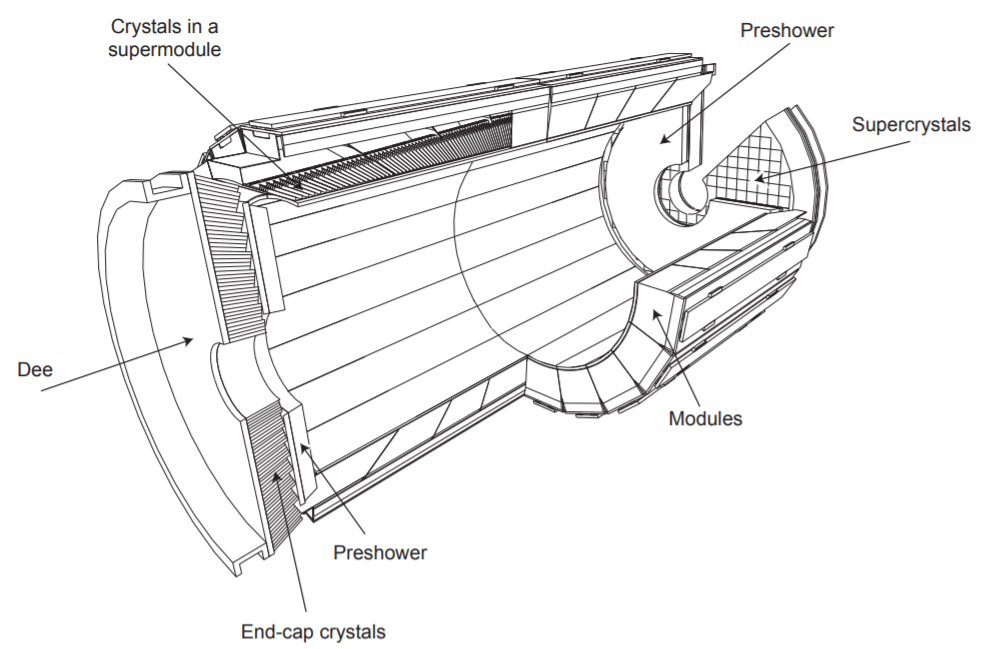
\includegraphics[width=0.7\linewidth]{Figures/ECAL_layout}
 	\caption{Schematic of ECAL. Reprint from \cite{Collaboration_2008}}
 	\label{fig:ecallayout}
 \end{figure}
 
 
The high density (8.28 g/cm$^{3}$), short radiation length ()

The ECAL is a hermetic homogeneous calorimeter containing 75848 lead tungstate (PbWO$_{4}$) crystals used for the detection and measurement of photon and electron energies.  The choice of PbWO$_{4}$ was made for its high density 
This is done via detection of scintillation light produced


It consists of 75848 lead tungstate (PbWO$_{4}$) crystals with 61200 of those mounted in a central barrel section (EB) and the remaining 14648 divided evenly between two endcaps (EE) \cite{Collaboration_2008}.  In front of each endcap is a pre


\section{Hadronic Calorimeter}

\section{Muon System}

